% !TEX root = main.tex
\newpage

\section{1D density advection-diffusion problem}~\label{App_1D}
\subsection{Description of the problem}

An initial exploration is conducted on a one-dimensional application to assess the filter performance. We define the following one-dimensional $2\pi$-periodic convection-diffusion problem such as
\begin{equation*}
	\frac{\partial u}{\partial t}(z,t) + v \frac{\partial u}{\partial z}(z,t)  = \visc \frac{\partial^2 u}{\partial z^2}(z,t),
\end{equation*}
with $z$ the spatial coordinate, $v$ a constant velocity and $\visc$ a constant diffusion coefficient.
For the following application, the reference solution will use $v = \refv$ and $\visc = \refvisc$ as parameters.
We define the $2\pi$-periodic heat kernel in one dimension, such as

\begin{equation*}
	\phi(u, s) = \sum_{k=-\infty}^{\infty} \frac{1}{\sqrt{4 \pi s}} \exp{\left(-\frac{{(u - kL)}^2}{4s} \right)}.
\end{equation*}where $L=2\pi$ the periodic length

Considering an initial condition characterized by a Gaussian shape expressed as $u^{gt}(z, 0) = \phi(z-z_0, Dt_0)$, where $\zz$, $t_0 = \frac{\sigma_0^2}{2D}$, and $\sigz$, we derive the comprehensive analytical solution utilizing the Green equation solution
\begin{equation*}
	u^{gt}(z, t) = \phi(z- v t - z_0, \visc (t+t_0)).
\end{equation*}The analytical solution is succinctly described as a Gaussian function, characterized by a mean that moves at the advection velocity and a standard deviation proportional to $t$ and $D$. This solution is visually depicted in Figure~\ref{fig:1d_analytical} across various assimilation time frames.

\begin{figure}[ht]
	\centering
	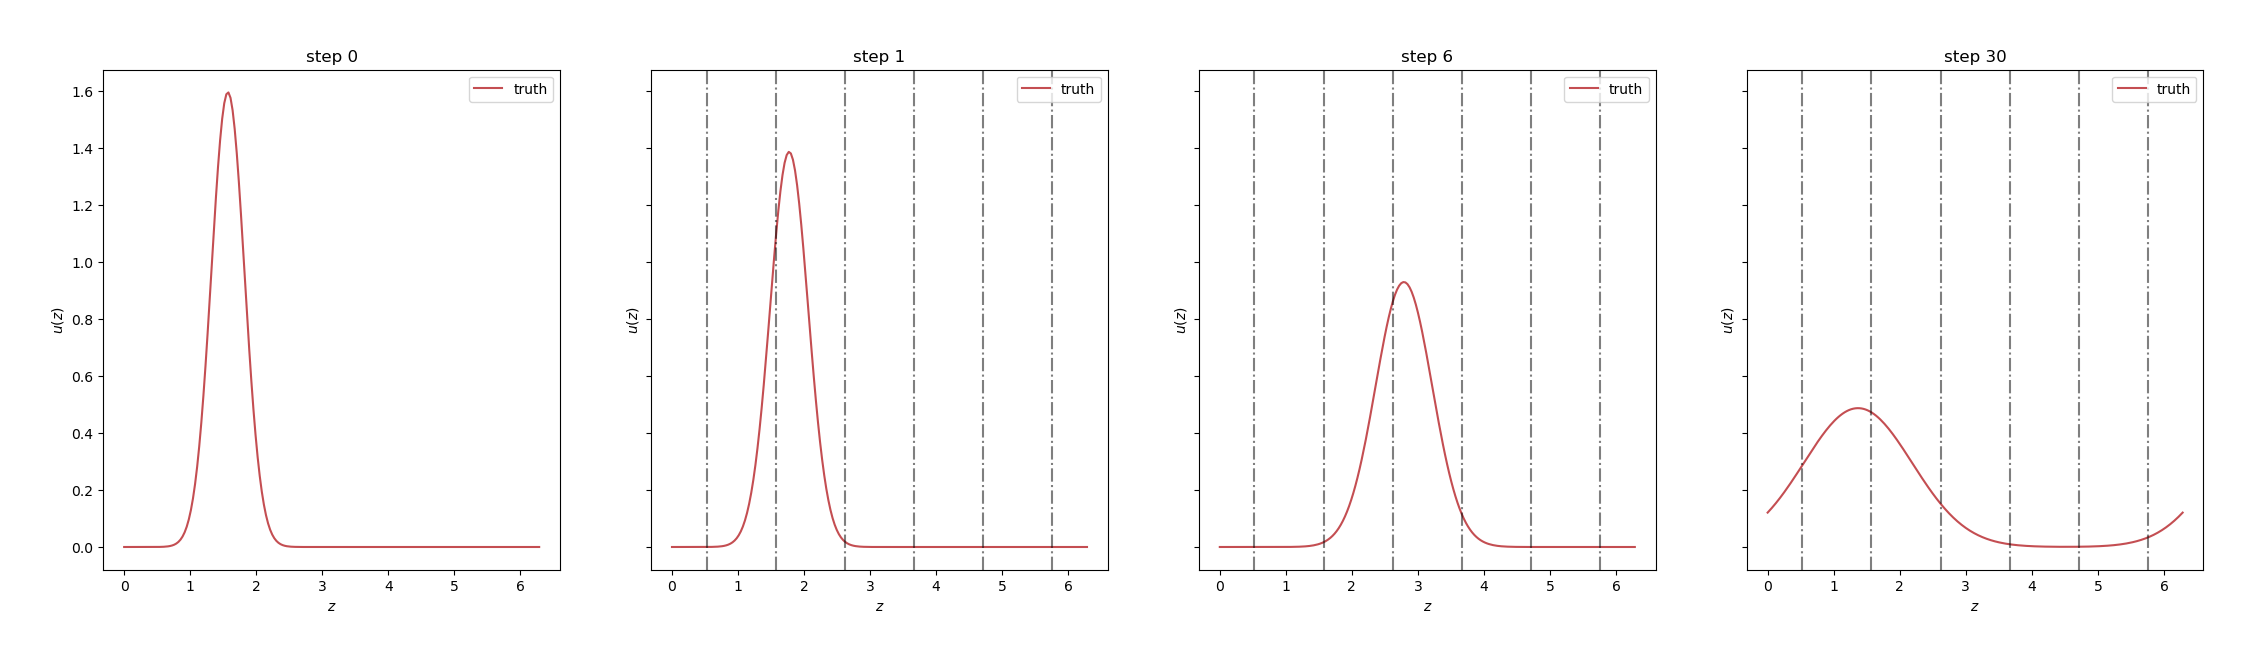
\includegraphics[width=\linewidth]{images/app1d/analytical_solution.png}
	\caption{The analytical solution of the convection-diffusion problem evolves over time, with the final snapshot revealing a complete spatial period.}
	\label{fig:1d_analytical}
\end{figure}

Following a Lagrangian perspective by tracking a fluid particle of position $z_p$ and intensity $U_p$, the equation becomes

\begin{equation*}
	\frac{dz_p}{dt} = v(z_p, t), \quad \frac{dU_p}{dt} = D \frac{d^2 U_p}{dz^2}
\end{equation*}

For solving the convection-diffusion scheme, we employ the two steps of the viscous splitting algorithm outlined in Section \ref{App_2D}. Initially, we address the equation for non-diffusive advection
\begin{equation*}
	\frac{dz_p}{dt} = v(z_p, t), \quad \frac{dU_p}{dt} = 0
\end{equation*}

and subsequently, we apply the diffusion equation
\begin{equation*}
	\frac{dz_p}{dt} = 0, \quad \frac{dU_p}{dt} = D \frac{d^2 U_p}{dz^2}
\end{equation*}

The advection is taken into account by updating the position of the particle with an Euler explicit scheme. %For a time step $dt$, the particle location become $z_p(t+dt) = z_p(t) + dt v$.
On the other hand, we use a redistribution method called the Particle Strength Exchange Method (PSE)~\cite{degond_1989,cottet_1990} to approximate the laplacian term $\frac{d^2 U_p}{dz^2}$.

Such as, the intensities $U_p$ are updated using the following formula
\begin{equation*}
	U_p = U_p + \varepsilon^{-1} \sum_{q} (U_q - U_p) \phi_g^P(z_q - z_p).
\end{equation*}with $\varepsilon$ the smoothing length of the Gaussian periodic kernel define as $ \phi^P_g = \sum_{n=-\infty}^{+\infty} \phi_g(r - n L)$.

For the periodic boundary problem described in section \ref{App_1D}, we define an equivalent kernel function $\phi^P_g = \sum_{n=-\infty}^{+\infty} \phi_g(r - n L)$, \\ . All the kernel properties are still verified on a single period.

Our particle-based model employs a discretization of \npart{} particles with a size of $h = \frac{L}{N_{\text{part}}}$ and a smoothing length of $\varepsilon = 1.3 h$.
For the sake of comparison, we solve the convection diffusion equation with a explicit (?) central finite difference scheme discretized on a regular grid with \ngrid{} nodes.

\subsection{Assimilation parameters and ensemble generation}

We conduct $N_{\text{assim}} = 30$ assimilation steps at evenly spaced intervals until the final time $t_f = 2 \frac{L}{v}$. During each assimilation step, the field $u^{gt}$ is observed at six regularly spaced positions $x_{\text{obs}}$. The observational data is subject to additive noise, denoted as $\eta \sim \mathcal{N}(0, \sigma_y \bm{I}_5)$, where $\sigma_y = \sigmaY$ and $\bm{I}_5$ represents the identity matrix.

All filters undergo testing on an identical initial prior ensemble of size $N = 25$ members, characterized by Gaussian shapes that are shifted and scaled. The mean of the ensemble is drawn from $Z_m \sim \mathcal{N}(\meanZm, \sigmaZm)$, while the standard deviation is drawn from $S_m \sim \mathcal{U}(\smLow, \smUp)$.
In the particle-based simulation, fields are discretized using regularly spaced particles that are shifted. Intensity values are obtained by fitting an interpolation operator like in Section~\ref{interpOp} to the particle intensity.
The parameter $\varepsilon_{\text{mass}}$ is introduced as a cutoff for particle selection, allowing for the definition of varying numbers of particles for each simulation. The differentiation in particle support poses challenges during the interpolation phase in the Part-EnKF.
Velocity $v$ is sampled from $v \sim \mathcal{N}(\vmean, \vstd)$, and diffusion $D$ is sampled from $D \sim \mathcal{U}(\Dlow, \Dup)$. The sample and initial state are illustrated in Figure~\ref{fig:initial_gen}.
Simultaneously, a standard Ensemble Kalman Filter (EnKF) update is applied to the nodal variables to construct the reference filter Grid-EnKF which use a grid-based model.

\begin{figure}[ht!]
	\centering
	\begin{subfigure}{0.49\textwidth}
		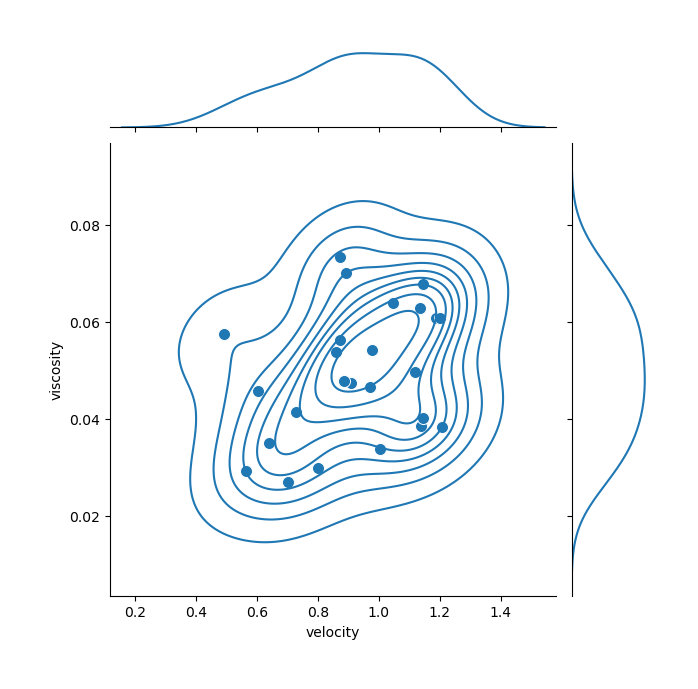
\includegraphics[width=\textwidth]{images/app1d/parameters.png}
	\end{subfigure}
	\hfill
	\begin{subfigure}{0.49\textwidth}
		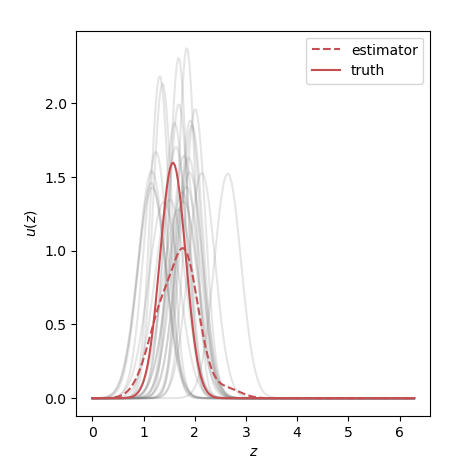
\includegraphics[width=\textwidth]{images/app1d/initial_state.png}
	\end{subfigure}
	\caption{On the left the initial parameters sample, $v$ in abscissa and $D$ in ordinate. On the right is the initial ensemble state.}
	\label{fig:initial_gen}
\end{figure}

For grid-based simulation, the fields of each member are interpolated at the node locations. In this way, the ensemble generated is still the same for the sake of comparison.
Finally, we define the relative $L_2$ error as

\begin{equation}~\label{eq:L2_error}
	e_{L_2} =\frac{ \frac1\nens \sum_{i = 1}^{\nens} \left(\int_\Omega \left(u^{gt}(z) - u_i(z)\right)^2 dz\right)^{1/2}}{\norm{u}_{L_2}}
\end{equation}~where $u_i$ denote the $i$-th member of the ensemble and $\norm{u}_{L_2}$ denote the $L_2$ norm of $u^{gt}$. We compute the parameter error with a norm-2 as $e_{\theta} = \frac{\frac1\nens \sum_{i = 1}^{\nens}  (\norm{\theta - \theta_{EnKF}}_2^2)^{1/2}}{\norm{\theta_{EnKF}}_2}$.

\subsection{Results}

We begin the comparison of the different filters by refraining from calibrating the parameters of the model. The filters exclusively update the state, treating the unknown parameters as a source of uncertainty for the model. The two filters outlined in the Method section~\ref{Methods} and the Eulerian filter are compared with the reference filter based on a grid discretization.
In figure \ref{fig:1d_error_time}, we appreciate a similar agreement for all the filters, except for Particle-EnKF, with a reduced number of particles in the support.

\begin{figure}
	\centering
	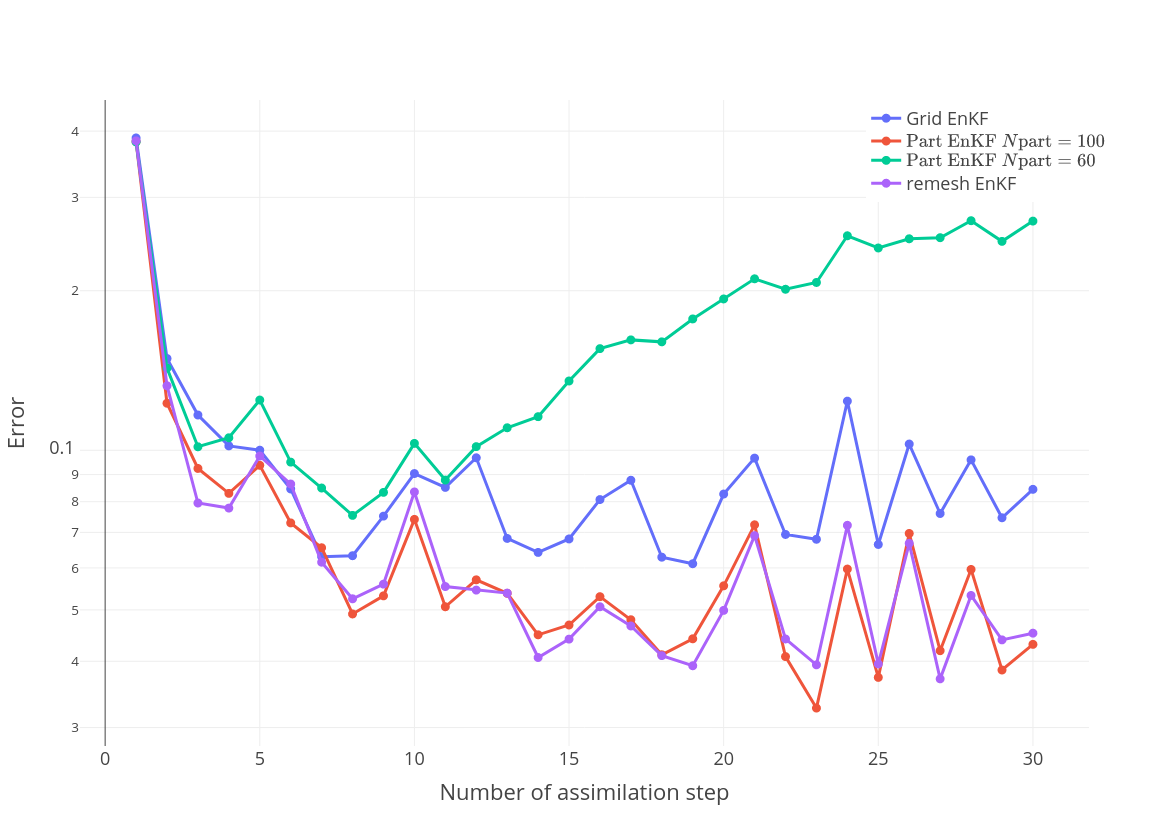
\includegraphics[width=0.75\textwidth]{images/app1d/wo_calibration/state_error.png}
	\caption{State error with respect to assimilation time step.}
	\label{fig:1d_error_time}
\end{figure}

% Faire référence à cette figure
\begin{figure}
	\centering
	\begin{subfigure}{\textwidth}
		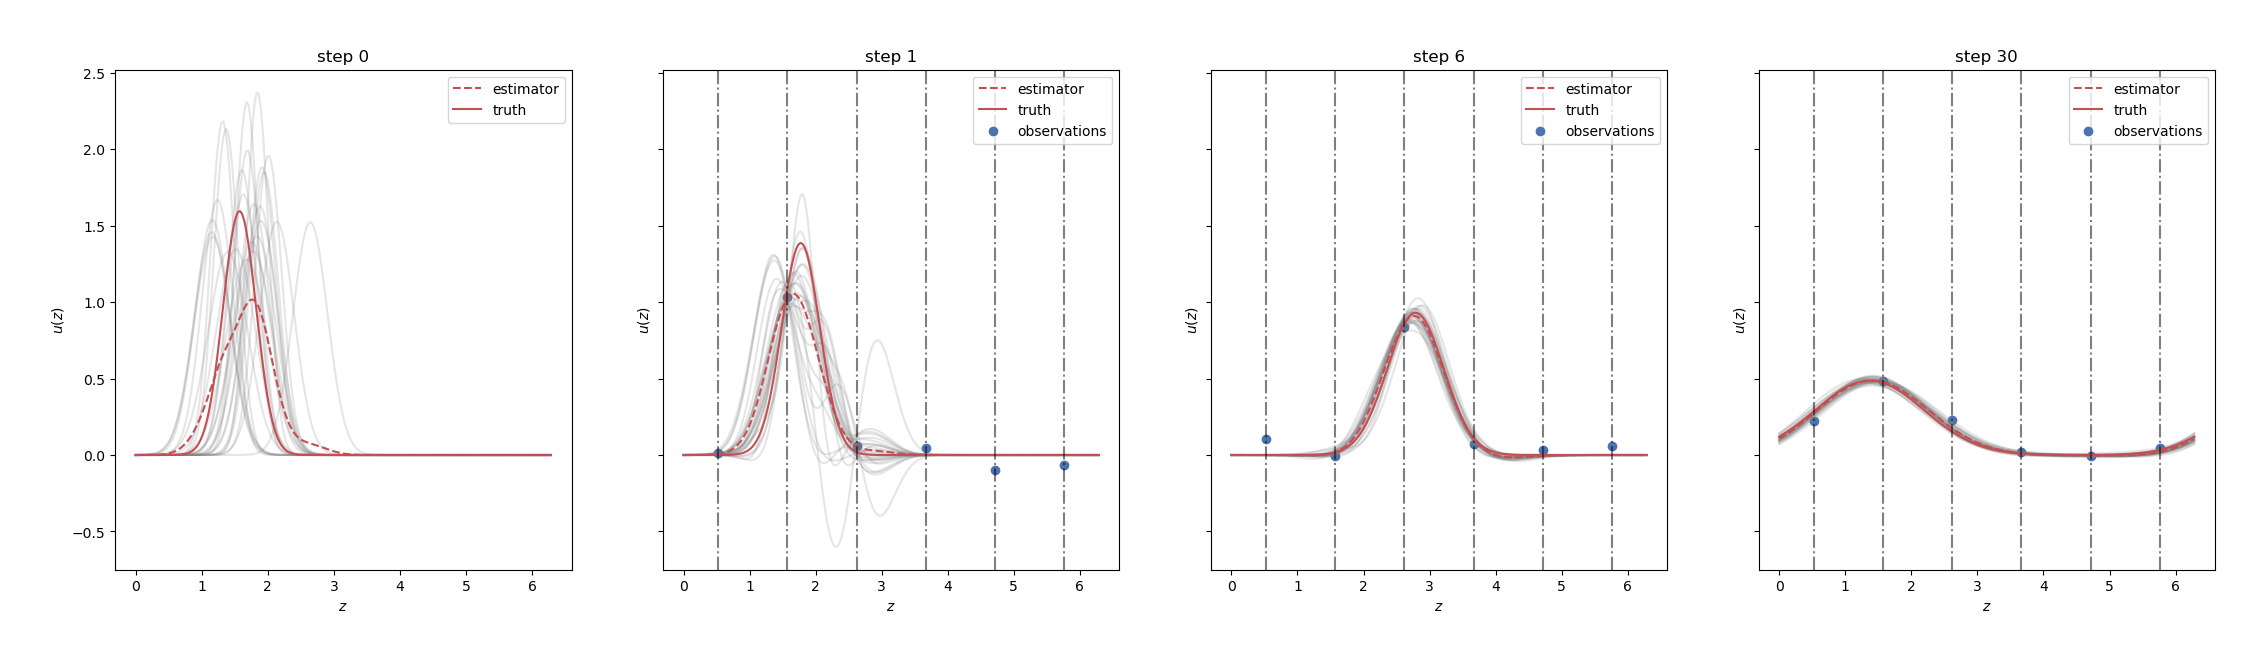
\includegraphics[width=\textwidth]{images/app1d/wo_calibration/remesh_EnKF.png}
	\end{subfigure}
	\caption{Data assimilation comparison over different filters. From top to bottom, with Grid Filter, RemeshEnKF, PartEnKF with $N_{part}=100$, and PartEnKF with $N_{part}=60$.}
\end{figure}
\newpage

The primary issue arises from the regression on non-overlapping support, where the regression struggles to fit the analysis solution defined on a more considerable space support. This leads to heightened variability, particularly in the tail of the distribution. Addressing this common challenge in RBF Regression \cite{fornberg_flyer_2015} involves increasing the Ridge penalization coefficient, a parameter we choose through cross-validation Ridge regression.
Even with a more stable regression, it remains a projection of the analysis solution onto the forecast support. It is imperative to increase the number of particles to achieve a better approximation of the analysis solution using the particle approximation operator in Section~\ref{interpOp} or the regression operator in Section~\ref{regressionOperator}.
We validate this assumption by varying the initial support of particles. Quantitatively, as observed in Figure~\ref{error_support}, the error decreases with an increase in the number of particles. Moreover, qualitatively examining the snapshot on the right reveals that the solution closely aligns with the reference.

\begin{figure}
	\centering
	\begin{subfigure}{0.39\textwidth}
		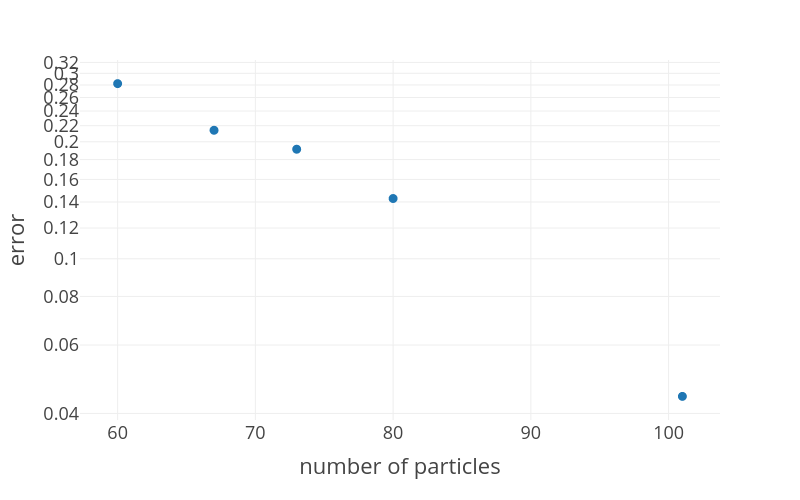
\includegraphics[width=\textwidth]{images/app1d/error_support/error_support.png}
		\label{error_support1}
	\end{subfigure}
	\hfill
	% Revoir figures en plotly
	\begin{subfigure}{0.29\textwidth}
		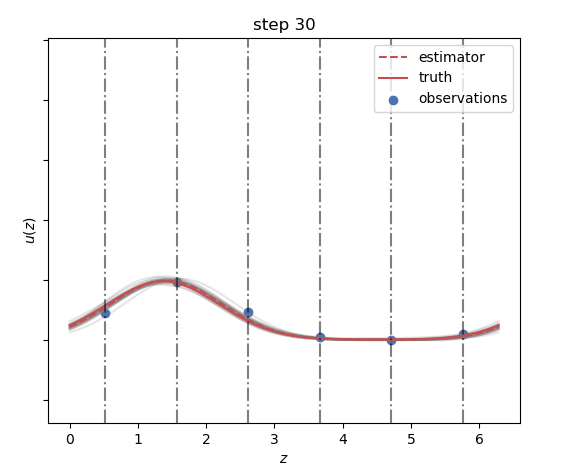
\includegraphics[width=\textwidth]{images/app1d/error_support/ok.png}
		\label{error_support2}
	\end{subfigure}
	\hfill
	\begin{subfigure}{0.29\textwidth}
		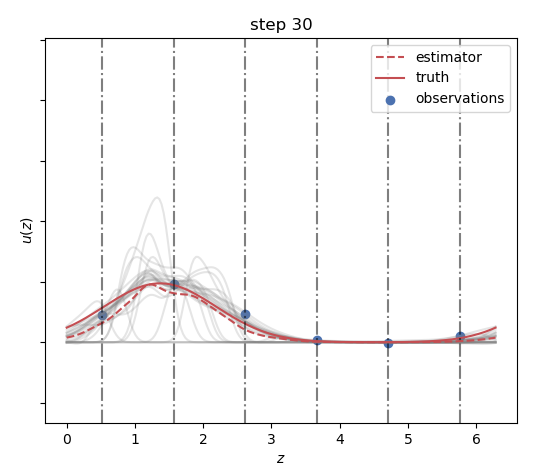
\includegraphics[width=\textwidth]{images/app1d/error_support/not_ok.png}
		\label{error_support3}
	\end{subfigure}
	\caption{Left: Error with respect to particle support size, Middle: Final step for a support of 100 particles, Right: Final step for a support of 60 particles.}
	\label{error_support}
\end{figure}
However, Adding particles in a more complex solution is a challenging task. Indeed, a good spacing between particles and the density of particles has to be preserved. In this case, we advise defining criteria for the error of the reconstruction. Instead of adding particles, we advise generating a new, regularly spaced grid of particles to reconstruct the solution.

In conclusion, this example underscores the Remesh-EnKF filter capability to yield results comparable to the classical EnKF applied to a grid model. Additionally, it highlights the Part-EnKF's capability in assimilating on a particle discretization while also emphasizing the importance of addressing spatial discrepancies between members, which can pose challenges in solution reconstruction. The computation of solution error reconstruction provides a straightforward criterion for remeshing a member and applying the analysis solution approximation.

\subsection{Expanded state}

In the case of an expanded state, we extend the update to parameters by introducing the variable $\theta = (v, D)$ in the state definition. This approach allows the calibration of these quantities.
Figure \ref{calib4} displays the marginal distribution of parameters over time obtained with Remesh-EnKF. The velocity and diffusion exhibit well-estimated values, indicated by unbiased means and a reduction in variability.

\begin{figure}[ht]
	\centering
	\begin{subfigure}{0.49\textwidth}
		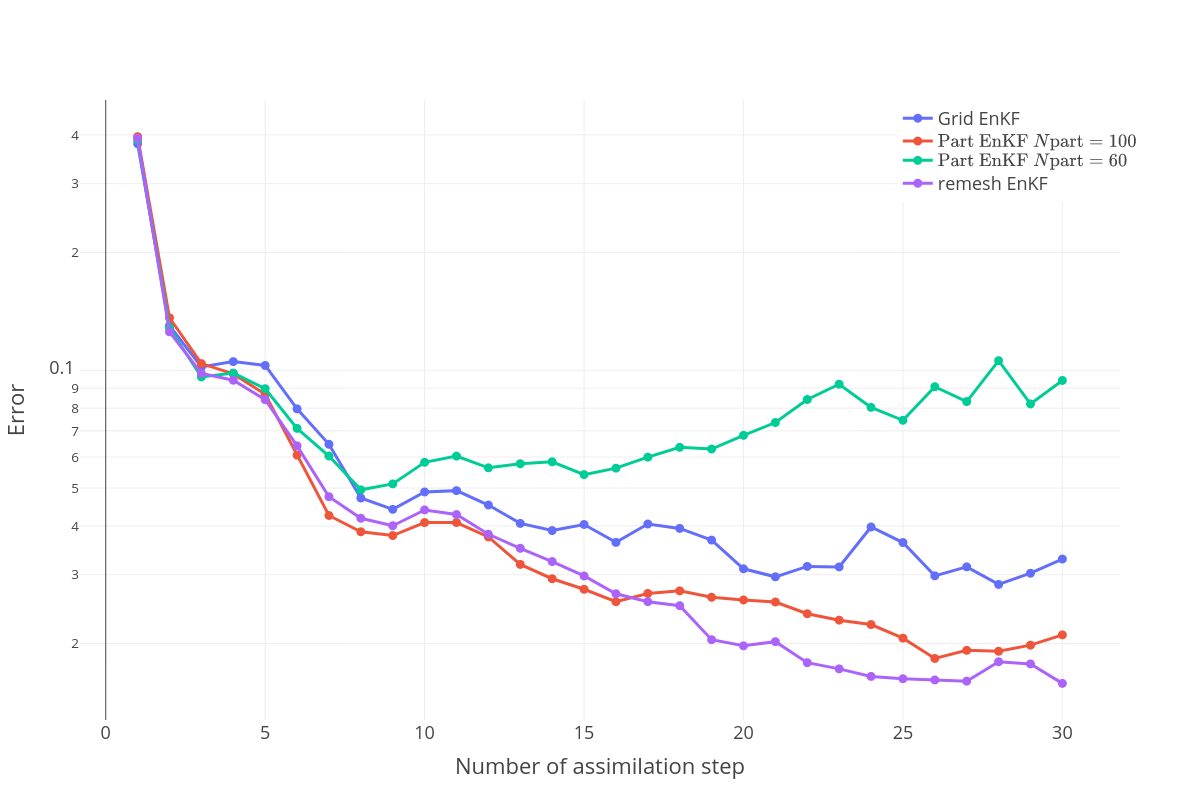
\includegraphics[width=\textwidth]{images/app1d/w_calibration/state_error.png}
		\caption{}
		\label{calib1}
	\end{subfigure}
	\hfill
	\begin{subfigure}{0.49\textwidth}
		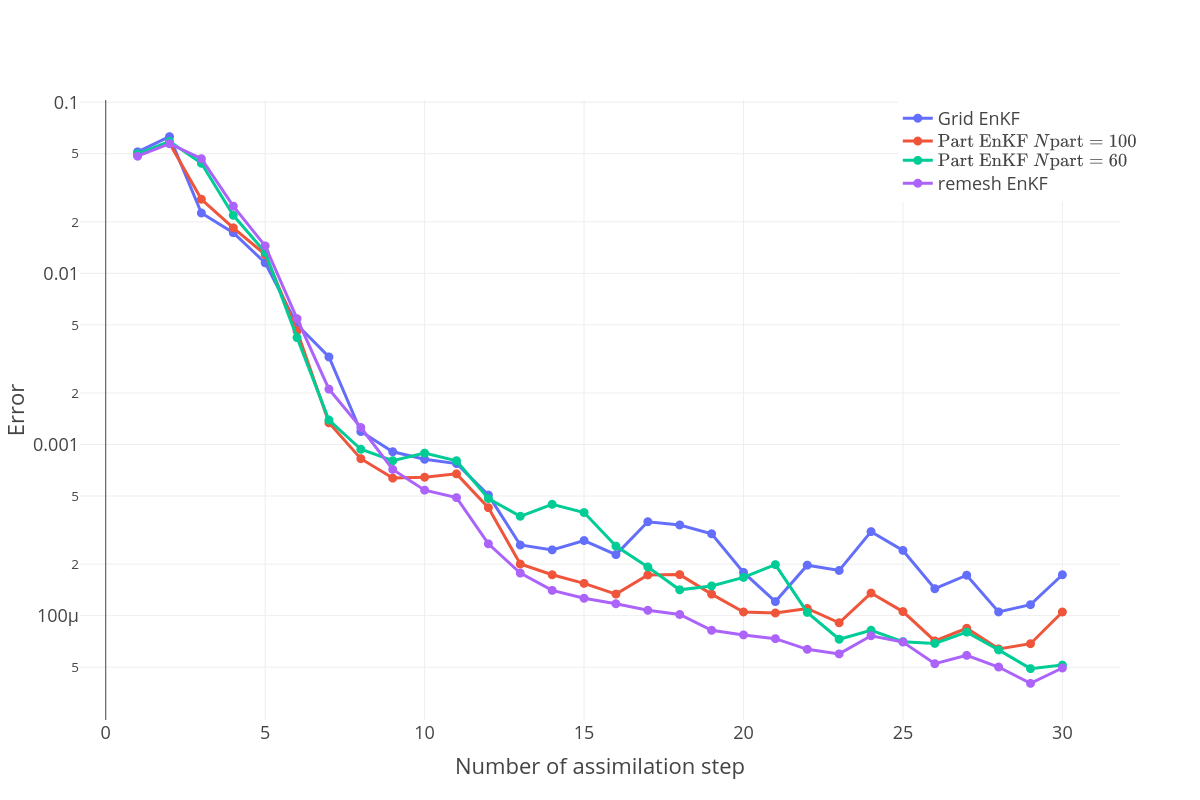
\includegraphics[width=\textwidth]{images/app1d/w_calibration/velocity_error.png}
		\caption{}
		\label{calib2}
	\end{subfigure}
	\vfill
	\begin{subfigure}{0.49\textwidth}
		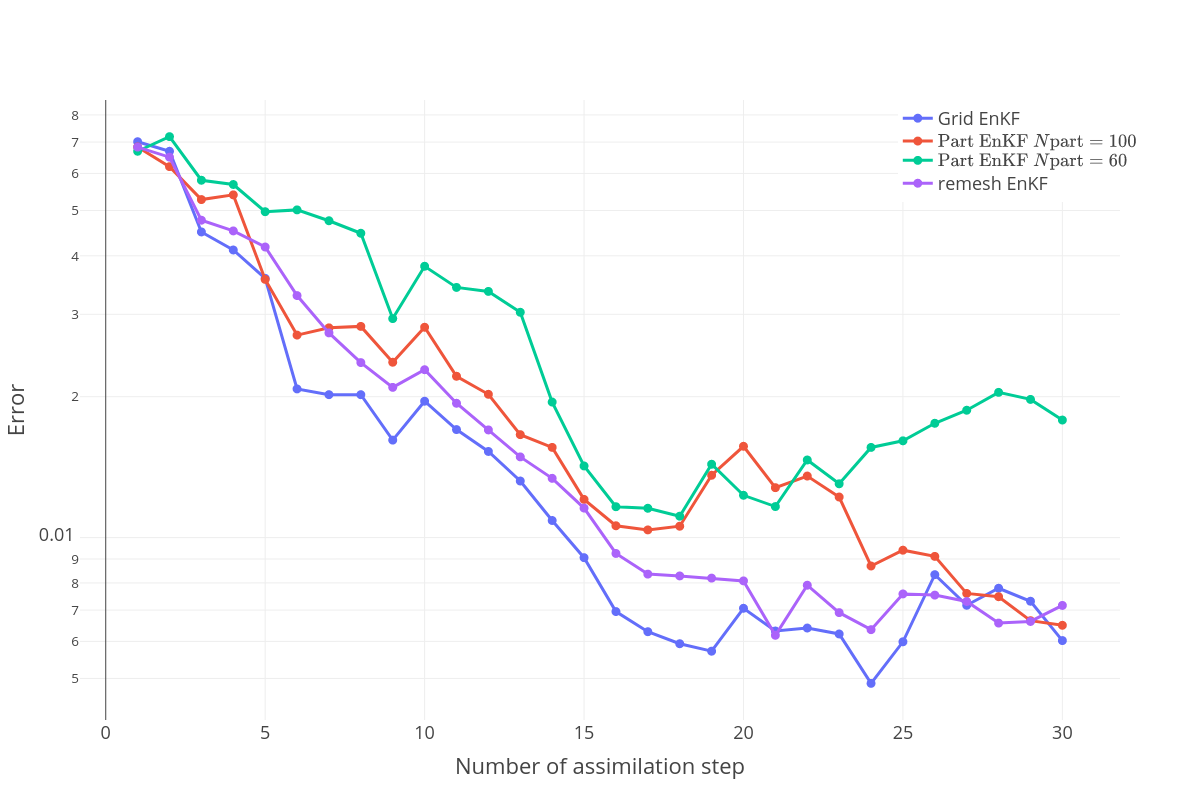
\includegraphics[width=\textwidth]{images/app1d/w_calibration/viscosity_error.png}
		\caption{}
		\label{calib3}
	\end{subfigure}
	\caption{In \subref{calib1}, \subref{calib2}, \subref{calib3} respectively state, velocity, and viscosity errors with respect to the assimilation time step.}
\end{figure}

\begin{figure}[ht]
	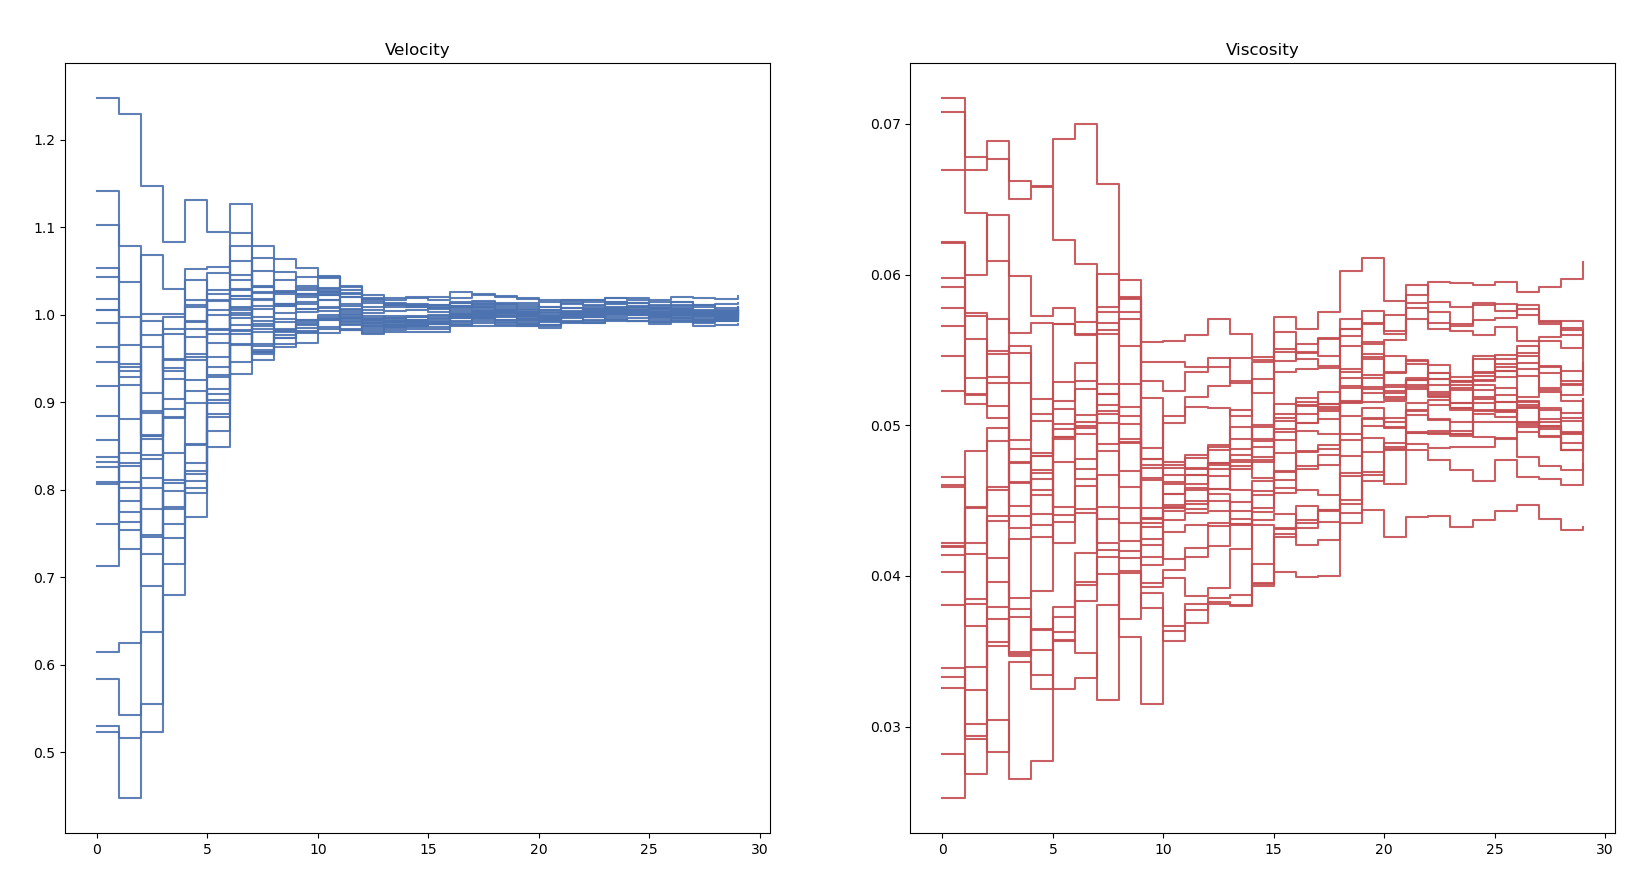
\includegraphics[width=\textwidth]{images/app1d/w_calibration/remesh EnKF_params.png}
	\caption{Marginal distribution of velocity (left) and viscosity (right) over time (Remesh-EnKF).}
	\label{calib4}
\end{figure}

Quantitatively, we also observe a reduction of error of the estimation of the state in \ref{calib1}, the estimate of the velocity \ref{calib2}, and the estimate of the diffusion \ref{calib3}.

Indeed, even though the state estimation was already well accurate in Figure \ref{fig:1d_error_time}, the state estimation further improves here, thanks to the calibration of the model parameters. Updating the parameters allows for adjusting the model to the observed data, thereby enhancing the accuracy of the state estimation. This underscores the significance of parameter calibration in achieving more precise results in the context of data assimilation.
It is noteworthy that even in the worst-case scenario of the Part-EnKF, the estimation of parameters remains accurate, indicating a good understanding of the dynamic behavior of the problem.

\newpage